
\chapter{Results}
This chapter should encompass your data analysis and findings. Additionally, include relevant tables, figures, and citations to support your results and interpretations. Here is a suggested list of topics to discuss:

  \section{Experiments and Tests}
  Describe the experiments conducted to assess the performance of your project. Explain how you collected and processed the data.
  
  \section{Data Visualization}
  Create visual representations of the results (e.g., scatter plots, bar charts). Interpret the visualizations and relate them to the research questions.
  
  \section{Limitations}
  Acknowledge any limitations in the data or analysis. Explain how these limitations may have influenced the results.

\section{Experiments and Tests}
Durante el transcurso de este proyecto, se han realizado una serie de experimentos con el objetivo de conseguir el mayor rendimiento para el simulador quantico de moléculas. Una parte importe de la simulación quantica es la decisión para las interfaces del calcula de las funciones de coste. Estas funciones son las que se tendrán que optimizar para conseguir el estado y la geometria optima de esa molécula. Normalmente, la interfaz mas eficaz para esta tarea es la JAX, ya que utiliza la aceleración de hardware mediante la GPU, que suelen ser mas eficaces y rapidas para encontrar el punto optimo de la función de coste. Después de ejecutar dos codigos de funcionaminto identico, con lo que lo unico que modificamos fue la interfaz de calulo, nos dimos cuenta de algo sorprendente. La interfaz de calculo de JAX, que se ejecutaba en la GPU, era mas lenta que la interfaz de calculo de autograd, que se ejecutaba en la CPU. Este resultado fue sorprendente, ya que la GPU suele ser mas eficaz para este tipo de tareas. Para asegurarnos de que no era un error en el codigo, ejecutamos el mismo codigo en diferentes maquinas, y el resultado fue el mismo. Por lo tanto, decidimos seguir con la interfaz de calculo de autograd, ya que era mas rapida y eficaz para este tipo de tareas.

Ejecutamos la misma optimización, unicamente modificando la interfaz, y nos guardamos los tiempos de ejecución de las distintas funciones que contenia el codigo y los guardamos en un archivo. A continuación, mostramos los resultados de los distintos tiempos de ejecución de las distintas simulaciones.

\begin{figure}[H]
  \centering
  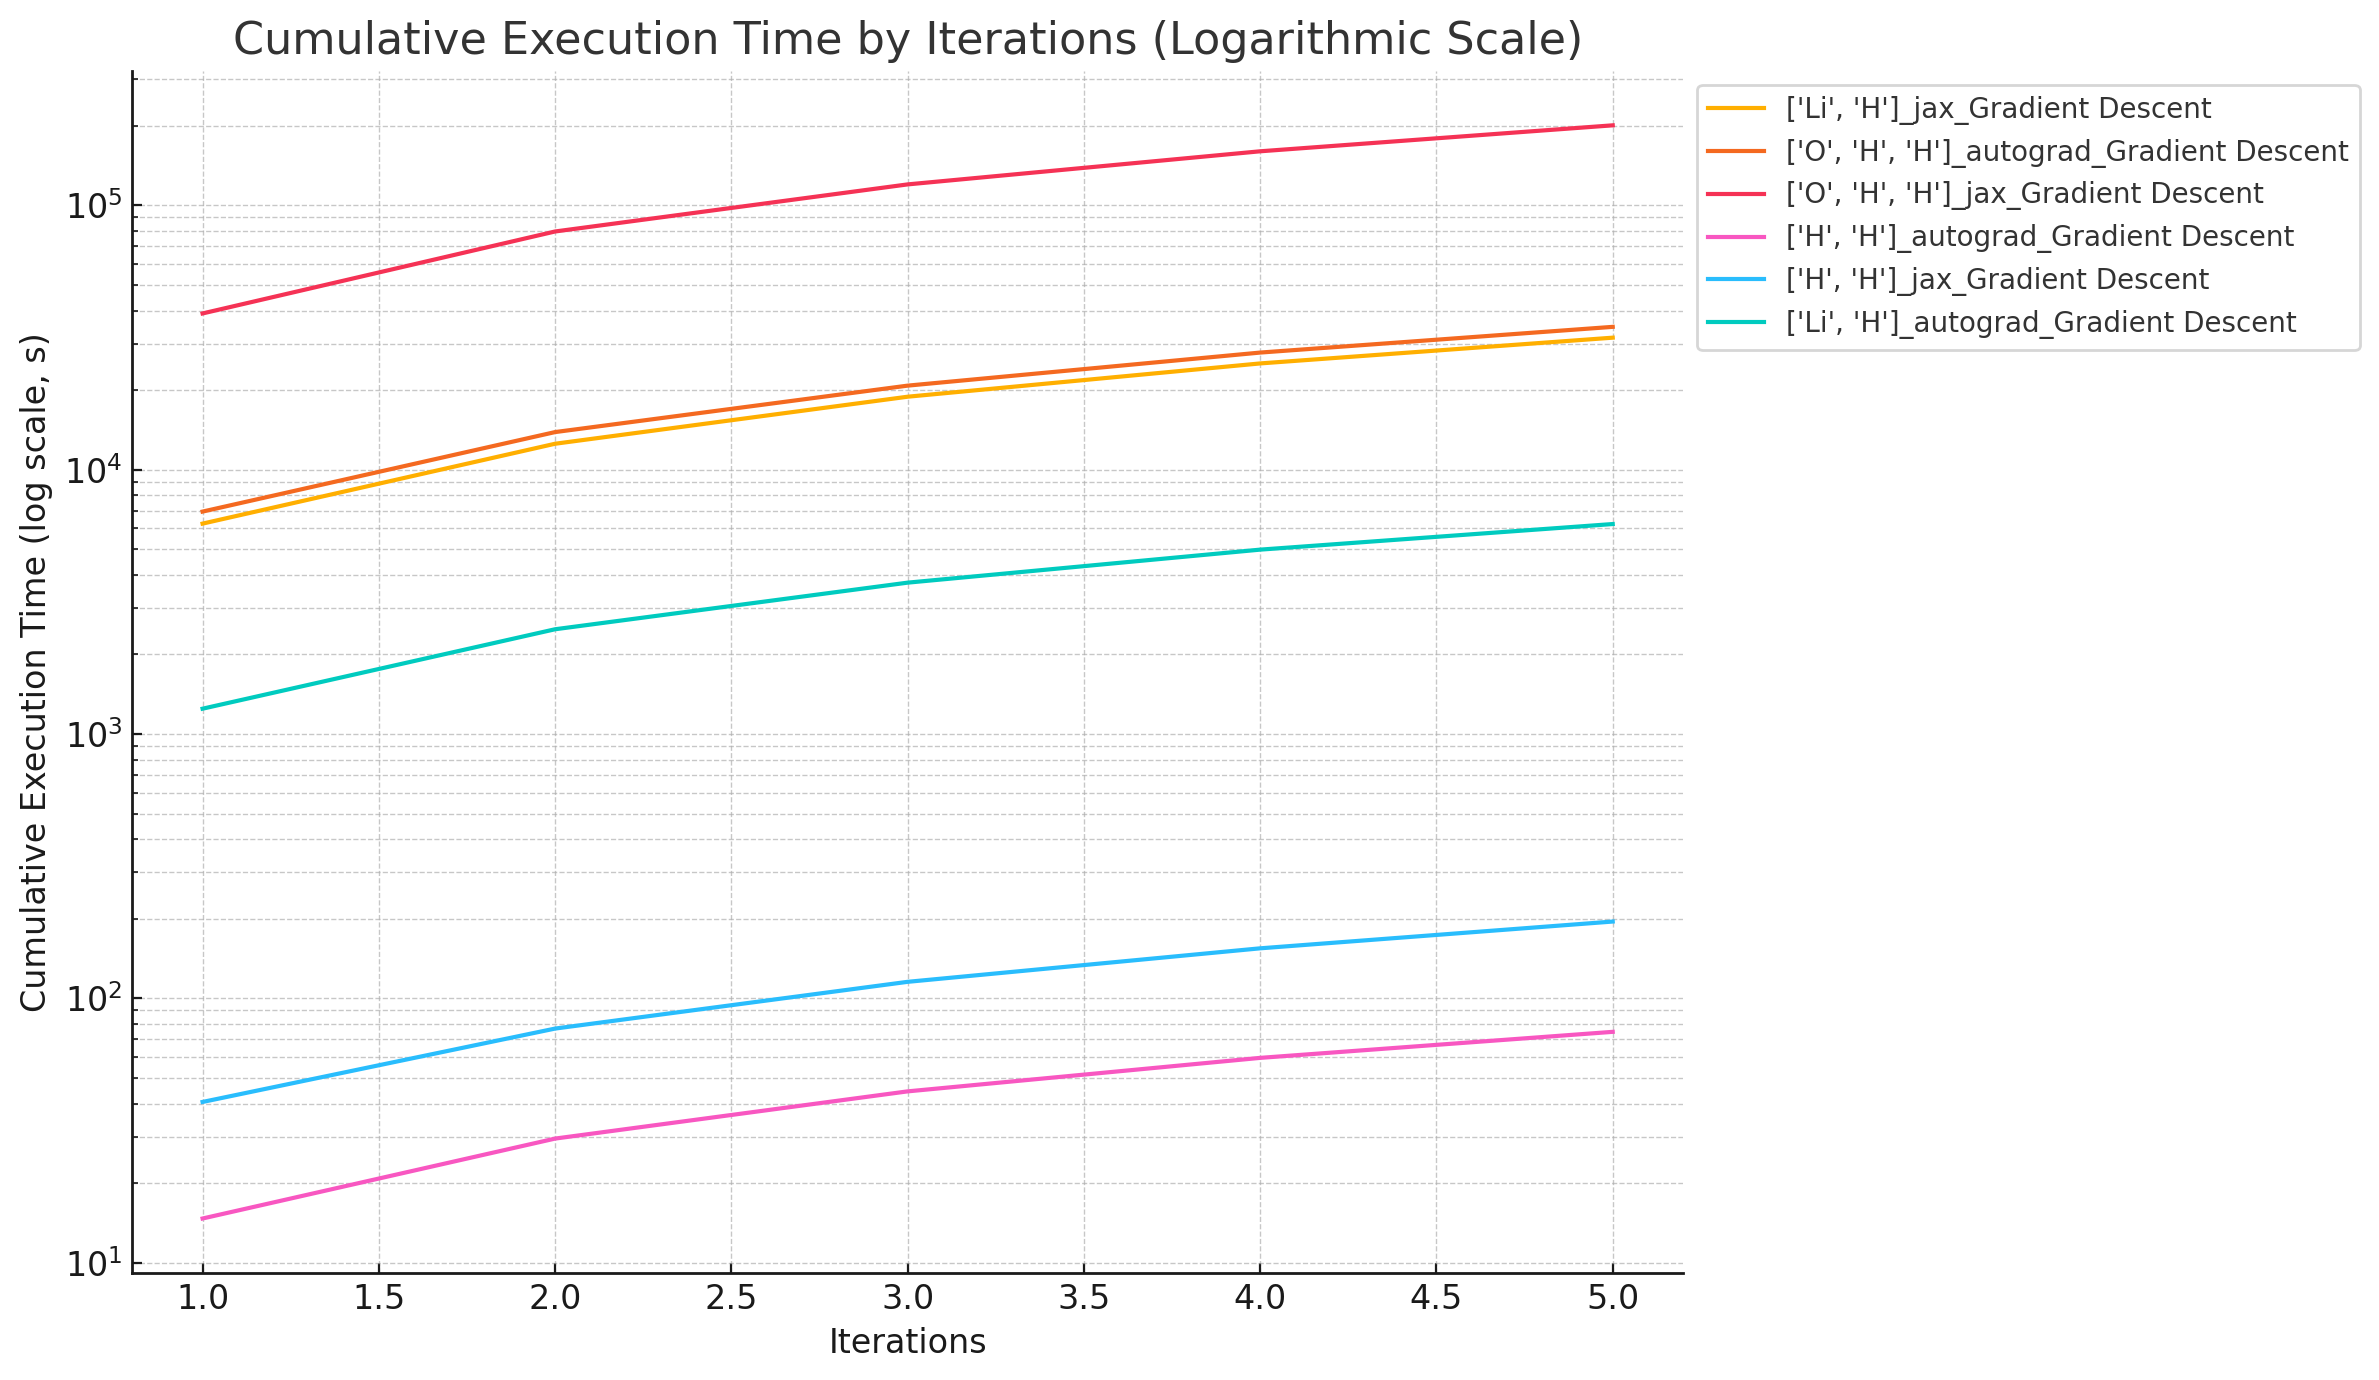
\includegraphics[width=0.8\textwidth]{img/time_iterations.png}
  \caption{Tiempo de ejecución de las distintas moleculas segun su iteración en la simulación.}
  \label{fig:time_iterations}
\end{figure}

Como se puede observar en la figura, en todos los casos, el tiempo de ejecución de la simulación es menor en la interfaz de autograd que en la interfaz de JAX. Si hacemos una media del tiempo total de ejecución de las simulaciones, obtenemos que la interfaz JAX, va un 74.92\% mas lenta que la interfaz de autograd. Otro dato tambien interestante es que si nos fijamos en el porcentaje de tiempo que pierde la interfaz de JAX, nos damos cuenta que a medida que la complejidad de la interfaz aumenta (es decir, a medida que aumenta el numero de atomos de la molecula), el porcentaje de tiempo que pierde la interfaz de JAX disminuie, esto nos da una pista del porque de estos resultados.

La segunda grafica que generamos fue la del tiempo de computo en cada parte de nuestro codigos. Para cada simulación, hicimos un seguimiento del tiempo que tardaba la ejecución en cada parte del código, donde se efectuaba el cambio de interfaz. A continuación, mostramos los resultados de los distintos tiempos de ejecución de las distintas simulaciones, los tiempos son acumulados. Para una mejor visualización, si quereis mas detalles sobre los tiempos de ejecución de cada parte del código, los puedes encontrar en el apartado de data.

\begin{figure}[H]
  \centering
  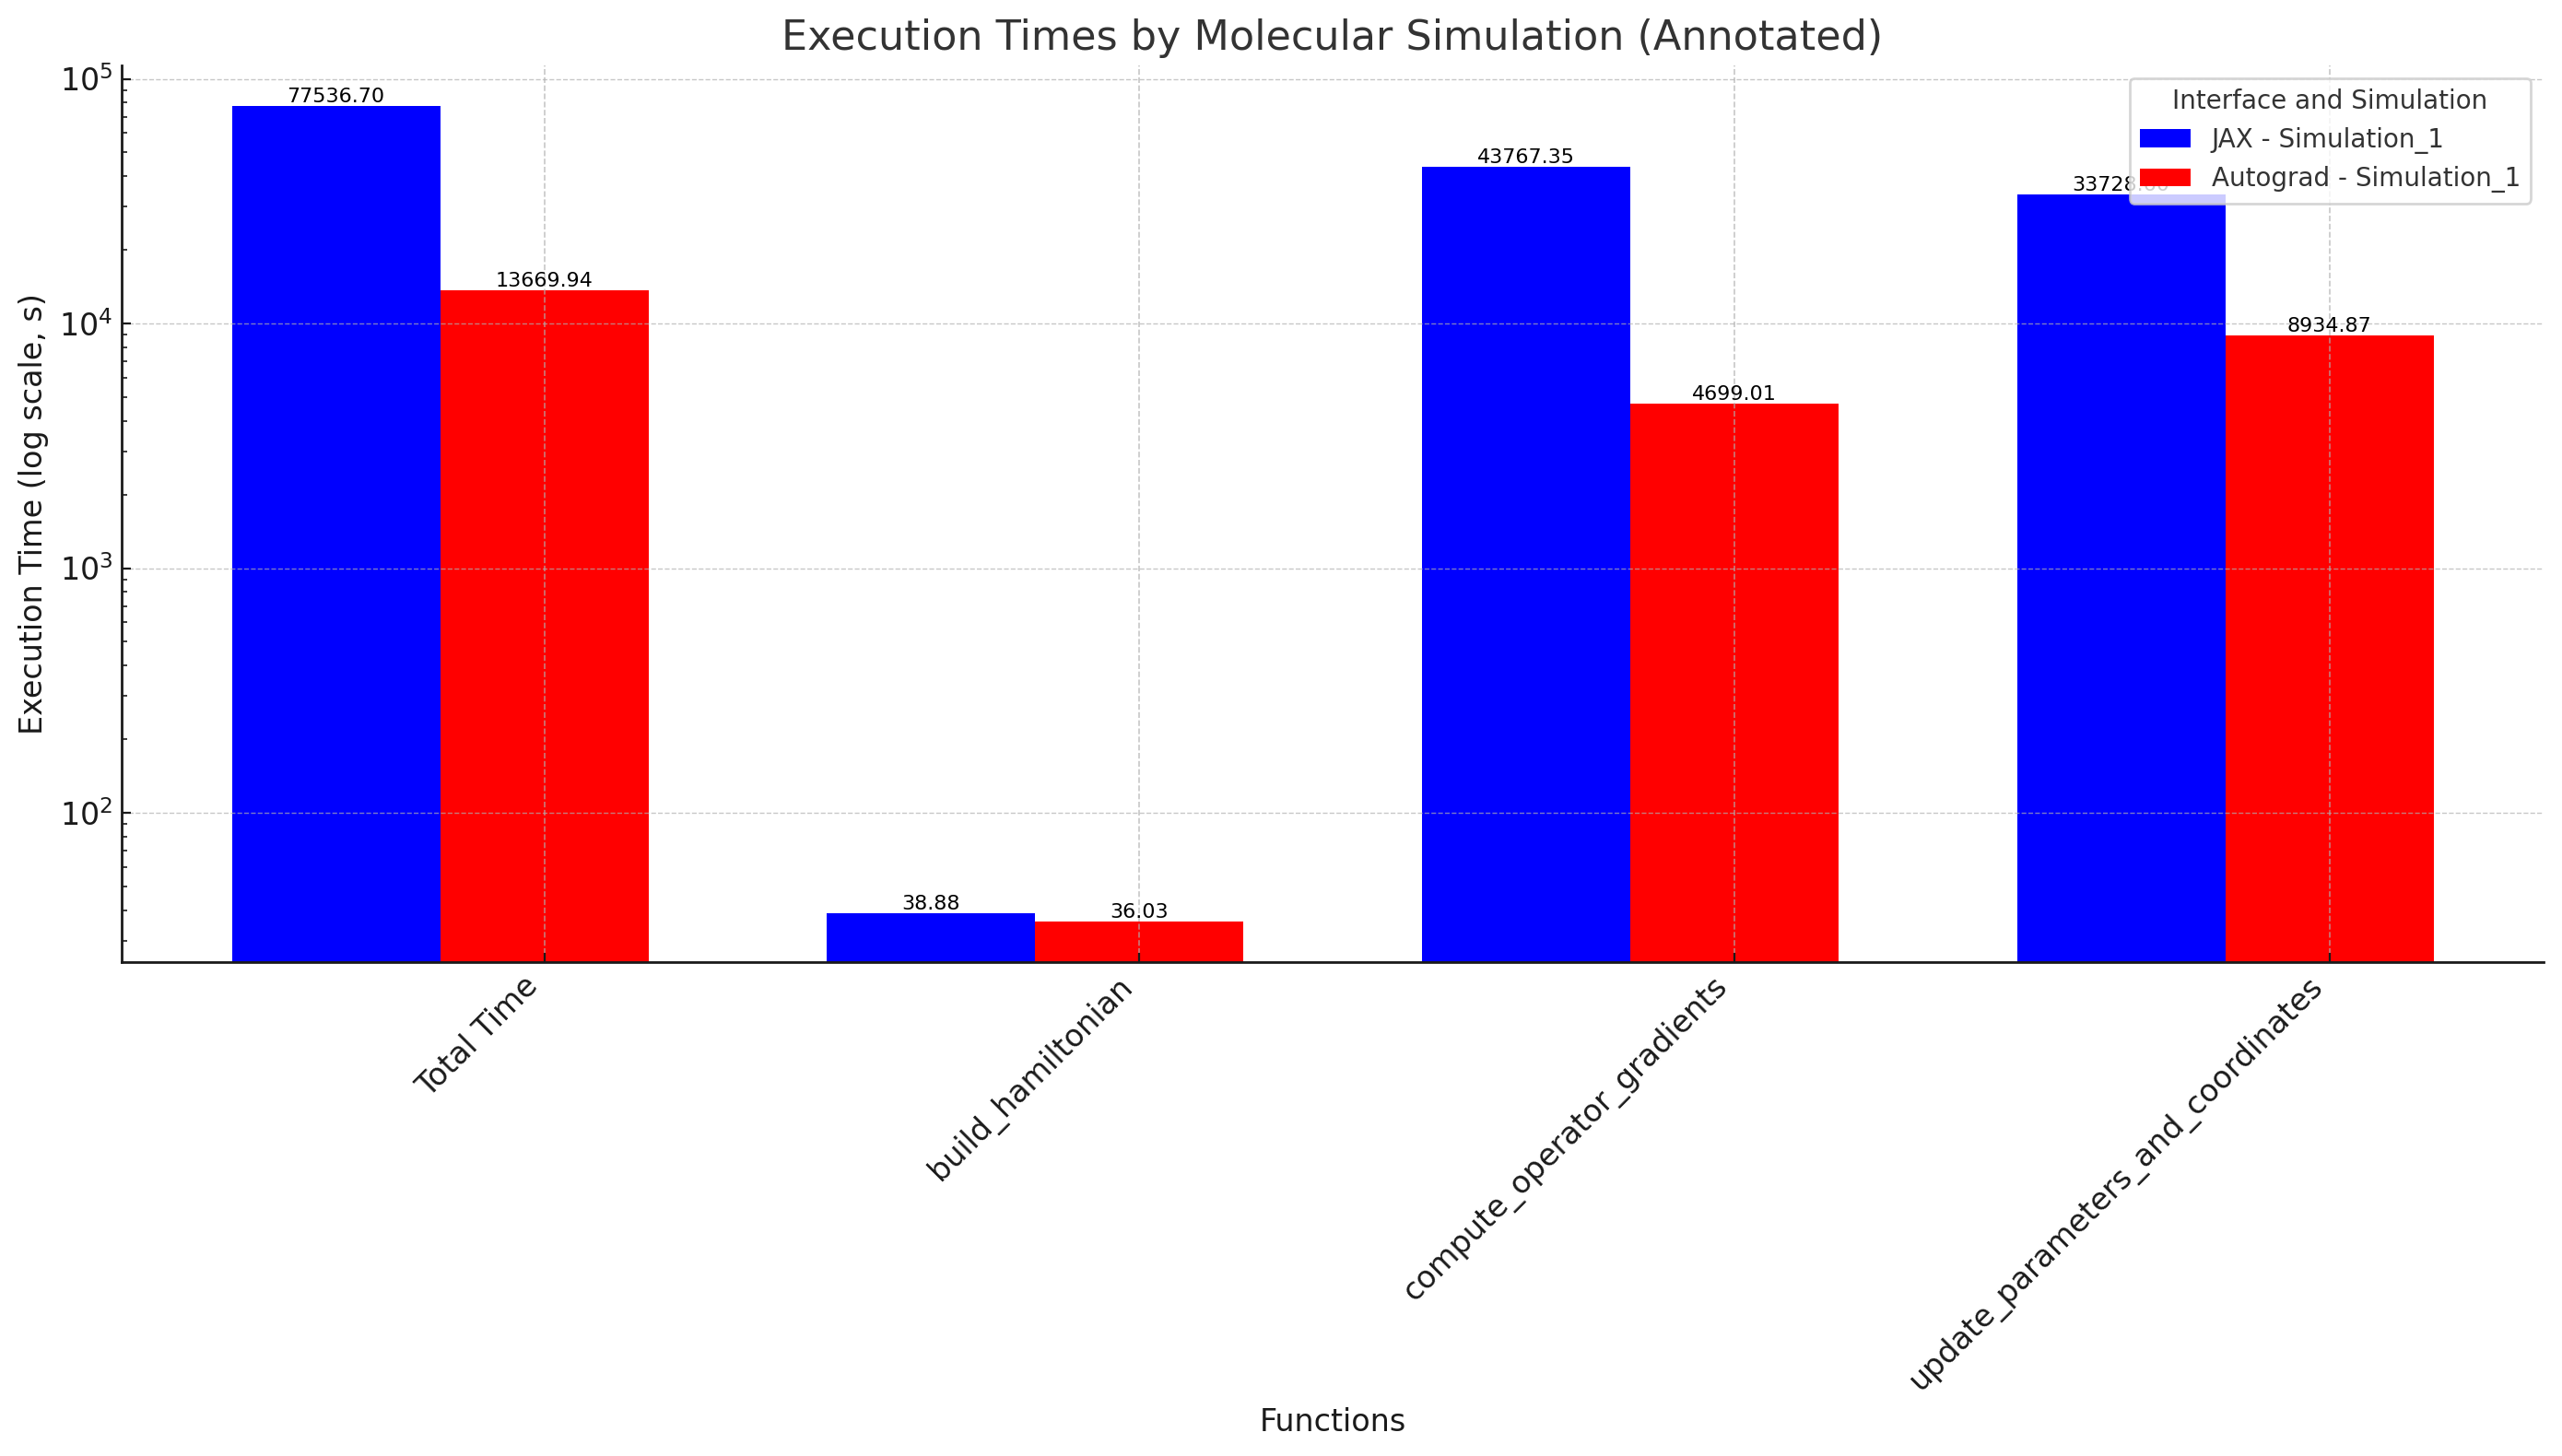
\includegraphics[width=0.8\textwidth]{img/time_functions.png}
  \caption{Tiempo de ejecución en distintas partes del codigo.}
  \label{fig:time_functions}
\end{figure}

Como se puede observar en la grafica, de igual manera que en la grafica anterior, la interfaz JAX, es mas lenta en todos los aspectos, de igual manera, obtenemos que en todas las partes del codigoñ. La diferencia de tiempo de casi todas las simulaciones, se debe al hoverhead de las simulaciónes. Se observa como a medida que el numero de transacciónes de información, dicho de igual manera, a medida que el numero de componentes que se calculan en la CPU, que estos se han de hacer inevitablemente ya que PennyLane no ofrece soporte para crear el hamiltoniano de la molecula en la GPU, el tiempo de ejecución de la interfaz de JAX aumenta, ya que el tiempo de transmisión de toda la información, posteriormente, no se gana en la GPU. Entonces, se observa que el calculo de gradientes de la funcion de coste, es la parte del codigo que mas le afecta este hoverhead, aumentando el tiempo de computo un 91.68\% para la interfaz de JAX.

La parte del codigo, que se encarga de hacer el paso de optimización de la geometria molecular y de los parametros, también recibe un incremento en su timepo de computo de un 67.04\% para la interfaz de JAX. Aun teniendo esto en cuenta, hay un factor que nos da la certeza de la razon por la cual la interfaz JAX, en esta implementación es mas lenta. Si nos fijamos en los datos, en la función de \textit{compute\_operator\_gradients}, a medida que el problema se hace mas complejo y que ha de tener mas valores para posteriormente calcular el gradiente de cada uno de los parametros, el tiempo de ejecución porcentualmente va decrementando. Resumiendo, que a medida que es mas complejo el problema, la interfaz JAX, se va haciendo mas eficaz, sin llegar a ser mas eficaz que autograd por eso. En cambio, en la función \textit{upgrade\_parameters\_and\_coordinates}, a medida que el problema se hace mas complejo, el tiempo de ejecución porcentualmente va aumentando Esto nos da una pista de que la diferencia de tiempo se debe al hoverhead que se produce en la transmisión de la información de la CPU a la GPU, ya que al tratarse de proceso de optimización poco complejos, pero con muchas iteraciones, que con la interfaz JAX, ha de cambiar todo el rato de la CPU a la GPU, el tiempo que se gana con la interfaz JAX, se pierde en la transmisión de la información.

Esta por esta razón, que finalmente la interfaz seleccionada para la implementación del simulador quantico molecular, fue la interfaz de autograd.
\subsection{Ansatz}
Uno de las modificaciones mas importante y que mas han afectado a nuestro codigo y al funcionamiento de nuestro codigo ha sido la elección del Ansatz. Nuestra propuesta ha sido implementar el UCSSD, un ansatz tipicamente utilizado para este tipo de simulaciones, ya que consigue incrementar el rendimiento de la simulación haciendo que tenga un mayor rendimiento. Para tener una idea de como mejora el rendimiento de nuestra simulación, hemos generado un ansatz con 20 niveles de profundidad y hemos comparado su rendimiento con el rendimiento de un ansatz UCSSD. 

%Hacer simulación para ver cual es la mejor profundidad para el ansatz

%Añadir imagen de la evolución de la energia en función de las iteraciones para distintos ansatz
Como se puede 
\subsection{Optimizador}
\paragraph{Selección del Optimizador}
Una vez seleccionada la interfaz de autograd, se procedió a la selección del optimizador. Para ello, se ejecutaron una serie de simulaciones con distintos optimizadores, y se observo la evolución de la energia del sistema en función de las iteraciones. Para ello, desenvolupamos, una manera de poder ejecutar simulaciones de las mismas moleculas con distintos optimizadores, y finalmente guardamos los resultados de los tiempos con la energia de la molecula en cada iteración, para cada molecula. 

%% Añadir imagen de la evolución de la energia en función de las iteraciones 
En la siguiente figura, podemos observar como para X iteraciones, el tiempo de ejecución no varia significativamente, lo que si que varia es el punto de convergencia que consigue cada uno de los optimizadores. En las figuras anteriores, se mostraban los distintos optimizadores para cada simulación y observamos que dependiendo de la molecula, el optimizador que mejor se adapta a la simulación es distinto. Esto era algo que ya se esperaba, ya que cada optimizador tiene sus ventajas y desventajas, y dependiendo de la molecula, el optimizador que mejor se adapta a la simulación es distinto. Aun asi, si el objetivo es encontrar un optimizador que funcione para la mayor parte de moleculas, hemos observado que el optimizador que mejor se adapta a la simulación es el Momentum. %Explicar mas en detalle el porque de la elección del optimizador basandonos en los resultados obtenidos.

\paragraph{Selección del Step Size}
Una vez seleccionado el optimizador, se procedió a la selección del step size. Para ello, se ejecutaron una serie de simulaciones previas para observar para que humbral de step size, se comportaba mejor el optimizador. Para ello se procedio a hacer un barrido de valores de step size que iban entre 0.1 a 0.7, y los resultados obtenidos son los siguientes.

%Añadir imagen de la evolución de la energia en función del step size

Como se puede observar en las tres imagenes, el rango de step size donde mejor funciona el optimizador es entre 0.1 y 0.3. Pasa algo curioso con la molecula H2, y es que el optimizador funciona mejor con un step size de 0.4, un valor relativamente alto. Esto se debe a que justamente, con este valor, el optimizador, por casualidad, consigue llegar a la condición de convergencia que hemos definido, %Explicar la condición de convergencia del codigo.

Aun asi, para observar mas concretamente, el valor de step size que mejor se adaptaba con nuestras simulaciones, decidimos volver a generar las simulaciones de las distintas moleculas con distintos step size, y observar la evolución de la energia en función de las iteraciones. Estos son los resultados.

%Añadir imagen de la evolución de la energia en función de las iteraciones para distintos step size

De igual manera que antes, se observa que dependiendo de la simulación, el valor de step size idoneo va variando segun el 


\subsection{Numero de Iteraciones}

Finalmente, una de los procesos donde mas tiempo se consume en la simulación es en la actualización de parametros y de las coordenadas, en esta ultima prueba lo que queremos conseguir es poder optimizar el numero de iteraciones que se actualizan los parametros y las coordenadas antes de volver a calcular el Hamiltoniano. Para ello, hemos generado una serie de simulaciones con distintos numeros de iteraciones, y hemos observado la evolución de la energia en función de las iteraciones.